% SPDX-License-Identifier: CC-BY-4.0
% DBOR specification - Dense Binary Object Representation
% Copyright (C) 2020 Daniel Lutz <dlu-ch@users.noreply.github.com>

\section{Values}
%%%%%%%%%%%%%%%%
\label{sec:values}

This section defines the representation of objects as bytes sequences - the core of DBOR.


\subsection{Overview (\DborValue)}
%%%%%%%%%%%%%%%%%%%%%%%%%%%%%%%%%%
\hypertarget{sec:def:Value}{}

% Relation between value and byte sequence
DBOR represents a sequence of \emph{objects} $O^*$ as a concatenation $B^*$ of their \emph{representations as byte
sequences} in such a way that the efficient reconstruction of $O^*$ from $B^*$ alone is possible by traversing $B^*$
in forward direction:
\begin{align*}
    \text{objects} & \quad\rightarrow\quad \text{byte sequence} \\[-2ex]
    -100, \text{"¡Olé!"}
        & \quad\mapsto\quad
    \ByteSequence{
        \underbrace{%
            \DborFirstByteHex{Number}{38}, \DborNextByteHex{4B}
        }_{\hskip-\textwidth\DborIntegerValue(-100)\hskip-\textwidth},
        %
        \overbrace{%
            \DborFirstByteHex{String}{67},
            \DborNextByteHex{C2}, \DborNextByteHex{A1},
            \DborNextByteHex{4F}, \DborNextByteHex{6C},
            \DborNextByteHex{C3}, \DborNextByteHex{A9},
            \DborNextByteHex{21}
        }^{\DborUtfEightStringValue(\text{"¡Olé!"})}
    }
\end{align*}
The representation is byte oriented and does not depend on word alignment or endianness.
The byte sequence of each encoded object describes its own size.

\medskip
The transformation of $O^*$ into $B^*$ is called \emph{encoding} (done by an DBOR encoder),
and the transformation of $B^*$ into $O^*$ is called \emph{decoding} (done by a DBOR decoder).

\medskip
DBOR \emph{focuses on the represented "value" of an object} to be encoded, not its type --
an unsigned $8$~bit number $42$ is no different from signed $64$~bit number $42$ in this view.%
\footnote{%
    This approach enables the definition and simple implementation of compatible interfaces between independent systems.

    Let's assume you need to send an unsigned $8$~bit number~$x$ as part of a command from a system~$A$ to
    an independent system~$B$ over a EIA-232 connection~$T$.
    \begin{enumerate}
        \item
        You implement the handling of $x$ as unsigned $8$~bit number on $A$ and $B$ and its transport over $T$
        as \DborIntegerValue{}.
        Then you release the systems~$A_1$ and $B_1$.

        \item
        You find out than $x$ sometimes needs $16$~bits.
        Therefore you adapt $A$ and $B$ to support this larger numbers and release $A_2$ and $B_2$.
    \end{enumerate}

    In the result, $A_1$ or $A_2$ can send the number $100$ to $B_1$ or $B_2$ and
    $A_2$ can send the number $1000$ to $B_1$ or $B_2$.
    When $B_2$ receives the number $1000$ from $A_2$, it rejects the command due to an argument larger than supported.
    All other combinations work as expected.
}
The byte sequence encoding an object is therefore called \emph{value}.

\medskip
DBOR groups objects of a common nature to be represented and encoded in a similar way by \emph{classes}
named \DborSyntaxIdent{}{\dots Value}.
The expression \DborIntegerValue($-100$) means the byte sequence that represents $-100$ as an instance of
class \DborIntegerValue{}:
\begin{equation*}
    \begin{array}{c}
        \DborIntegerValue(-100) \\
        = \ByteSequence{\DborFirstByteHex{Number}{38}, \DborNextByteHex{4B}}
    \end{array}
    \quad\text{is an instance of}\quad \DborIntegerValue
\end{equation*}
Each value identifies in its first byte the (concrete) class that it is an instance of.

\medskip
An abstract class like \DborNumberValue{} represents common traits of objects and can be used as placeholder for any
of its concrete subclasses (like \DborIntegerValue{} or \DborInfinityValue{} in this case).
The byte sequence \ByteSequence{\DborFirstByteHex{Number}{38}, \DborNextByteHex{4B}} "is a" \DborNumberValue{},
an \DborElementaryValue{}, and a \DborValue{} (all abstract classes).

\begin{figure}[H]
    \begin{quote}
        \noindent
        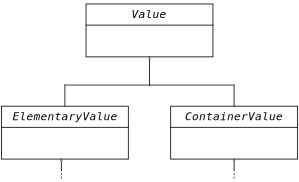
\includegraphics[scale=0.8]{classdiag_value}%
        \caption{Class hierarchy of values.}
        \label{fig:class:Value}
    \end{quote}
\end{figure}

See sections~\ref{sec:elementaryvalues} and \ref{sec:containervalues} for a complete list of (concrete) values.

\medskip
For some objects and classes, there is more than one representation of the object as an instance of the class;
The number $0.1$ can be represented as \DborDecimalRationalValue(1, -1) or \DborDecimalRationalValue(10, -2),
for example.
DBOR defines a \emph{canonical value} for each object and class to enable a unique representation.%
\footnote{
    This is important when a value is used as a key in a dictionary.
}


\subsection{\DborNoneValue}
%%%%%%%%%%%%%%%%%%%%%%%%%%%%%%
\label{sec:def:NoneValue}
\hypertarget{sec:def:NoneValue}{}

\paragraph{Representable objects}

A \DborNoneValue{} represents the absence of an actual object (like \texttt{null} or \texttt{None} in some
programming languages or NaN in IEEE-754:2008).
It is considered different from any object represented by a \DborValue*{} other than a \DborNoneValue.

\paragraph{Representation}

A \DborNoneValue{} is the \DborMinimalToken*($3$, $\HexNumber{1F}$).

\smallskip
\noindent
\begin{BeginParPenalty}
    Example:
    \begin{quote}
        \noindent
        \begin{tabular}{ll}
            \toprule
            Value & Representation \\
            \midrule
            \DborNoneValue & \ByteSequence{\DborFirstByteHex{None}{FF}} \\
            \bottomrule
        \end{tabular}
    \end{quote}
\end{BeginParPenalty}

\paragraph{Ambiguity, canonical value}

There is only one representation of a \DborNoneValue.
It is canonical.
Every \DborNoneValue{} is well-formed.


\subsection{Elementary values (\DborElementaryValue)}
%%%%%%%%%%%%%%%%%%%%%%%%%%%%%%%%%%%%%%%%%%%%%%%%%%%%%
\label{sec:elementaryvalues}
\hypertarget{sec:def:ElementaryValue}{}
\hypertarget{sec:def:NumberValue}{}
\hypertarget{sec:def:NumberlikeValue}{}
\hypertarget{sec:def:StringValue}{}

Elementary values are values that represent a single object with a meaning of its own (e.g. an integer).

\begin{figure}[H]
    \begin{quote}
        \noindent
        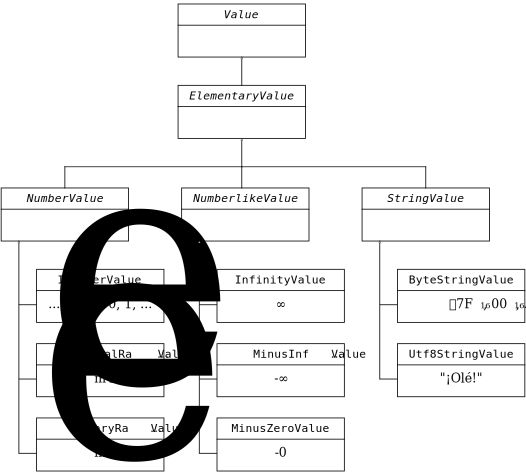
\includegraphics[scale=0.8]{classdiag_elementary}%
        \caption{Class hierarchy of elementary values.}
        \label{fig:class:ElementaryValue}
    \end{quote}
\end{figure}

Each \DborNumberValue{} represents a real number.

Each \DborNumberlikeValue{} represents an object that is no (real) number but can be compared to any real number and
to any \DborNumberlikeValue{}.


\subsubsection{\DborMinusZeroValue, \DborInfinityValue, \DborMinusInfinityValue}
%%%%%%%%%%%%%%%%%%%%%%%%%%%%%%%%%%%%%%%%%%%%%%%%%%%%%%%%%%%%%%%%%%%%%%%%%%%%%%%%%%%%%%%%%%%%%%%%%%%%%%%
\label{sec:def:MinusZeroValue}
\label{sec:def:InfinityValue}
\label{sec:def:MinusInfinityValue}
\hypertarget{sec:def:MinusZeroValue}{}
\hypertarget{sec:def:InfinityValue}{}
\hypertarget{sec:def:MinusInfinityValue}{}

\paragraph{Representable objects}

A \DborMinusZeroValue{} represents the "number" $-0$ in the sense of IEEE-754:2008 arithmetic.
It is considered larger than any object represented by a \DborNumberValue*{} with a negative numeric value and $< 0$.%
\footnote{%
    This reflects the idea of negative infinitesimal (\href{https://en.wikipedia.org/wiki/Hyperreal_number}{hyperreal}
    or \href{https://en.wikipedia.org/wiki/Surreal_number}{surreal}) numbers as members of an extension field
    of $\SetOfReals$.

    In IEEE-754:2008 arithmetic however (which introduces "non-numbers" primarily as an elegant means to make fast
    floating-point arithmetic more robust), $-0 = 0$ but $x / -0 \ne x / 0$ for finite $x \ne 0$;
    $-0$ and $0$ are treated as negative or positive infinitesimal numbers, respectively, in this operation.
}

\medskip
A \DborInfinityValue{} represents the "number" $\infty$ in the sense of IEEE-754:2008 arithmetic.
It is considered larger than any object represented by a \DborNumberValue*{}.

\medskip
A \DborMinusInfinityValue{} represents the "number" $-\infty$ in the sense of IEEE-754:2008 arithmetic.
It is considered smaller than any object represented by a \DborNumberValue*{}.

\paragraph{Representation}

A \DborMinusZeroValue{} is the \DborMinimalToken*($3$, $\HexNumber{1C}$).

An \DborInfinityValue{} is the \DborMinimalToken*($3$, $\HexNumber{1E}$).

A \DborMinusInfinityValue{} is the \DborMinimalToken*($3$, $\HexNumber{1D}$).

\smallskip
\noindent
\begin{BeginParPenalty}
    Examples:
    \begin{quote}
        \noindent
        \begin{tabular}{ll}
            \toprule
            Value & Representation \\
            \midrule
            \DborMinusZeroValue & \ByteSequence{\DborFirstByteHex{Numberlike}{FC}} \\
            \DborMinusInfinityValue & \ByteSequence{\DborFirstByteHex{Numberlike}{FD}} \\
            \DborInfinityValue & \ByteSequence{\DborFirstByteHex{Numberlike}{FE}} \\
            \bottomrule
        \end{tabular}
    \end{quote}
\end{BeginParPenalty}

\paragraph{Ambiguity, canonical value}

There is only one representation of a \DborMinusZeroValue,
\DborInfinityValue, and \DborMinusInfinityValue, respectively.
They are canonical.
Every \DborMinusZeroValue, \DborInfinityValue,
and \DborMinusInfinityValue{} is well-formed.


\subsubsection{\DborIntegerValue(\texorpdfstring{$v$}{v})}
%%%%%%%%%%%%%%%%%%%%%%%%%%%%%%%%%%%%%%%%%%%%%%%%%%%%%%%%%%
\hypertarget{sec:def:IntegerValue}{}

\paragraph{Representable objects}

An \DborIntegerValue{} can represent any number $v \in \IntegerInterval{-(N + 24)}{N + 23}$.

\smallskip
The minimum representable number is $-18\,519\,084\,246\,547\,628\,312$.
The maximum representable number is $18\,519\,084\,246\,547\,628\,311$.

\paragraph{Representation}

A number $v \in \IntegerInterval{0}{N + 23}$ is represented as \DborIntegerToken*(0, $v$).
A number $v \in \IntegerInterval{-(N + 24)}{0}$ is represented as \DborIntegerToken*(1, $-v - 1$).

\smallskip
\noindent
\begin{BeginParPenalty}
    Examples:
    \begin{quote}
        \noindent
        \begin{tabular}{ll}
            \toprule
            Value & Representation \\
            \midrule
            %
            \DborIntegerValue($0$)
                &  \ByteSequence{\DborFirstByteHex{Number}{00}} \\
            \DborIntegerValue($-1$)
                &  \ByteSequence{\DborFirstByteHex{Number}{20}} \\
            \DborIntegerValue($23$)
                &  \ByteSequence{\DborFirstByteHex{Number}{17}} \\
            \DborIntegerValue($24$)
                &  \ByteSequence{\DborFirstByteHex{Number}{18}, \DborNextByteHex{00}} \\
            \DborIntegerValue($-100$)
                &  \ByteSequence{\DborFirstByteHex{Number}{38}, \DborNextByteHex{4B}} \\
            \DborIntegerValue($\HexNumber{FF\,FF\,FF\,FF}$)
                &  \ByteSequence{\DborFirstByteHex{Number}{1B}, \DborNextByteHex{E7}, \DborNextByteHex{FE},
                   \DborNextByteHex{FE}, \DborNextByteHex{FE}} \\
            %
            \bottomrule
        \end{tabular}
    \end{quote}
\end{BeginParPenalty}

A non-empty byte sequence \ByteSequence{b_1, \ldots, b_n} is a \emph{well-formed} \DborIntegerValue{}
if and only if it is an \DborIntegerToken*(0, $w$) or an \DborIntegerToken*(1, $w$) for
a suitable $w \in \IntegerInterval{0}{N + 23}$

The sequence is an \emph{ill-formed} \DborIntegerValue{} if and only if it is not a well-formed
\DborIntegerValue{} but $b_1$ is the first byte of a \DborIntegerToken*(0, $w$) or
an \DborIntegerToken*(1, $w$).

\paragraph{Ambiguity, canonical value}

There is at most one representation of a \DborIntegerValue($v$) for any $v$.
It is canonical.


\subsubsection{\DborBinaryRationalValue(\texorpdfstring{$p$, $v$}{p, v})}
%%%%%%%%%%%%%%%%%%%%%%%%%%%%%%%%%%%%%%%%%%%%%%%%%%%%%%%%%%%%%%%%%%%%%%%%%
\hypertarget{sec:def:BinaryRationalValue}{}

\paragraph{Representable objects}

A \DborBinaryRationalValue{} can represent any number
\begin{equation}
    v = (-1)^s \cdot \sum_{i = -52}^0 m_i s^i \cdot 2^e
\end{equation}
with $s, m_i \in \{0, 1\}$, $e \in \IntegerInterval{2 - 2^{10}}{2^{10}}$ and $v \ne 0$.

The set of representable numbers comprises all normal and subnormal values of the IEEE-754:2008 type
\texttt{binary64} except $\pm 0$.

\smallskip
The maximum representable number is $(2 - 2^{-52}) \cdot 2^{2^{10}} \approx 3.595\,386 \cdot 10^{308}$.
The smallest positive representable number is $2^{-52} \cdot 2^{2-2^{10}} = 2^{-1074}
\approx 4.940\,656 \cdot 10^{-324}$.

\paragraph{Representation}

A number $(-1)^s \cdot (1 + M/2^p) \cdot 2^e$ with
\begin{align*}
    s & \in \{0, 1\} \\
    p & \in \{4, 10, 16, 23, 30, 37, 44, 52\} \\
    M & \in \IntegerInterval{0}{2^p - 1} \\
    e & \in \IntegerInterval{\max(0, p - 51) - 2^{r - 1} + 1}{2^{r - 1}} \\
    r & := 8 \lfloor p / 7 \rfloor + 7 - p
\end{align*}%
is represented as
\DborBinaryRationalToken*($p$, $0$, $s$, $M$, $e + 2^{r - 1} - 1$).

A number $(-1)^s \cdot M/2^p \cdot 2^{-1022}$ with $p := 52$, $s \in \{0, 1\}$ and
$M \in \IntegerInterval{1}{2^p - 1}$ is represented as \DborBinaryRationalToken*($p$, $1$, $s$, $M$, $0$).

\smallskip
\noindent
\begin{BeginParPenalty}
    For reference, here are the resulting combinations for all possible $p$:
    \begin{quote}
        \noindent
        \newcolumntype{R}{>{$}r<{$}}% package 'array'
        \begin{tabular}{R R R R >{\hspace{-.8em}$}c<{$\hspace{-.8em}} R R}
            \toprule
            k & r & p & & e && 2^{r - 1} - 1 \\
            \midrule
            0 &  3 &  4 & -3 & \ldots & 4 & 3 \\
            1 &  5 & 10 & -15 & \ldots & 16 & 15 \\
            2 &  7 & 16 & -63 & \ldots & 64 & 63 \\
            3 &  8 & 23 & -127 & \ldots & 128 & 127\\
            4 &  9 & 30 & -255 & \ldots & 256 & 255 \\
            5 & 10 & 37 & -511 & \ldots & 512 & 511 \\
            6 & 11 & 44 & -1023 & \ldots & 1024 & 1023 \\
            7 & 11 & 52 & -1022 & \ldots & 1024 & 1023 \\
            \bottomrule
        \end{tabular}
    \end{quote}
\end{BeginParPenalty}

\smallskip
\noindent
\begin{BeginParPenalty}
    Examples:
    \begin{quote}
        \noindent
        \begin{tabular}{ll}
            \toprule
            Value & Representation \\
            \midrule
            \DborBinaryRationalValue($4$, $\frac{1}{8}$)
                &  \ByteSequence{\DborFirstByteHex{Number}{C8}, \DborNextByteHex{00}} \\
            \DborBinaryRationalValue($10$, $-(2^{17} - 2^6)$)%
                \footnote{$-\left(1 + (1 - 2^{-10})\right) \cdot 2^{16}$}
                &  \ByteSequence{\DborFirstByteHex{Number}{C9}, \DborNextByteHex{FF}, \DborNextByteHex{FF}} \\
            \DborBinaryRationalValue($52$, $2^{-1022}$)
                &  $\ByteSequence{\DborFirstByteHex{Number}{CF},
                        \DborNextByteHex{00}, \DborNextByteHex{00}, \DborNextByteHex{00}, \DborNextByteHex{00},$ \\
                &  $    \DborNextByteHex{00}, \DborNextByteHex{00}, \DborNextByteHex{10}, \DborNextByteHex{00}}$ \\
            \DborBinaryRationalValue($52$, $2^{-1074}$)
                &  $\ByteSequence{\DborFirstByteHex{Number}{CF},
                        \DborNextByteHex{01}, \DborNextByteHex{00}, \DborNextByteHex{00}, \DborNextByteHex{00},$ \\
                &  $    \DborNextByteHex{00}, \DborNextByteHex{00}, \DborNextByteHex{00}, \DborNextByteHex{00}}$ \\
            \bottomrule
        \end{tabular}
    \end{quote}
\end{BeginParPenalty}

A non-empty byte sequence \ByteSequence{b_1, \ldots, b_n} is a \emph{well-formed}
\DborBinaryRationalValue{} if and only if
it is a \DborBinaryRationalToken*($p$, $o$, $s$, $M$, $E$) for suitable $p$, $o$, $s$, $M$ and $E$.

The sequence is an \emph{ill-formed} \DborBinaryRationalValue{} if and only if it is not a well-formed
\DborBinaryRationalValue{} but $b_1$ is the first byte of a
\DborBinaryRationalToken*($p$, $o$, $s$, $M$, $E$).

\paragraph{Ambiguity, canonical value}

There may be more than one representation of \DborBinaryRationalValue($p$, $v$) for any $v$.
Of these, the one with the smallest $p$ is the canonical value.%
\footnote{
    A \DborBinaryRationalValue($p$, $v$) is therefore canonical if and only if there is
    no \DborBinaryRationalValue($q$, $v$) with $q < p$.
    See \ref{sec:implementation:BinaryRationalValue:canonical} for an efficient way to check this.
}

For every \DborBinaryRationalValue($p$, $v$) with $p < 52$, there is also
a \DborBinaryRationalValue($p$, $v$) for any
$q \in \{4, 10, 16, 23, 30, 37, 44, 52\}$ with $q > p$.


\subsubsection{\DborDecimalRationalValue(\texorpdfstring{$m$, $e$}{m, e})}
%%%%%%%%%%%%%%%%%%%%%%%%%%%%%%%%%%%%%%%%%%%%%%%%%%%%%%%%%%%%%%%%%%%%%%%%%%
\hypertarget{sec:def:DecimalRationalValue}{}

\paragraph{Representable objects}

A \DborDecimalRationalValue{} can represent any number
\begin{equation}
    v = m \cdot 10^e
\end{equation}
with
\begin{align*}
    m & \in \IntegerInterval{-(N + 24)}{-1} \cup \IntegerInterval{1}{N + 23} \\
    e & \in \IntegerInterval{-(N + 8)}{-1} \cup \IntegerInterval{1}{N + 8}
\end{align*}

\smallskip
The minimum representable number is $-18\,519\,084\,246\,547\,628\,312 \cdot 10^{18\,519\,084\,246\,547\,628\,296}$.
The maximum representable number is $18\,519\,084\,246\,547\,628\,311 \cdot 10^{18\,519\,084\,246\,547\,628\,296}$.
The smallest positive representable number is $10^{-18\,519\,084\,246\,547\,628\,296}$.

\paragraph{Representation}

A number $m \cdot 10^e$ with with $m \in \IntegerInterval{-(N + 24)}{-1} \cup \IntegerInterval{1}{N + 23}$
and $e \in \IntegerInterval{-(N + 8)}{-1} \cup \IntegerInterval{1}{N + 8}$
is represented as \DborPowerOfTenToken*($e$) {\Concat} \DborIntegerValue*($m$).

\smallskip
\noindent
\begin{BeginParPenalty}
    Examples:
    \begin{quote}
        \noindent
        \begin{tabular}{ll}
            \toprule
            Value & Representation \\
            \midrule
            \DborDecimalRationalValue($1$, $-2$)
                &  \ByteSequence{\DborFirstByteHex{Number}{E9}, \DborNextByteHex{01}} \\
            \DborDecimalRationalValue($-123$, $100$)
                &  \ByteSequence{\DborFirstByteHex{Number}{D0},
                        \DborNextByteHex{5B}, \DborNextByteHex{38}, \DborNextByteHex{62}} \\
            \bottomrule
        \end{tabular}
    \end{quote}
\end{BeginParPenalty}

A non-empty byte sequence \ByteSequence{b_1, \ldots, b_n} is a \emph{well-formed}
\DborDecimalRationalValue{} if and only if
it is \DborPowerOfTenToken*($e$) {\Concat} \DborIntegerToken*($m$) for suitable $m \ne 0$ and $e$.

The sequence is an \emph{ill-formed} \DborDecimalRationalValue{} if and only if it is not a well-formed
\DborDecimalRationalValue{} but $b_1$ is the first byte of a \DborPowerOfTenToken*($e$).

\paragraph{Ambiguity, canonical value}

There may be more than one \DborDecimalRationalValue($m$, $e$) representing the same number $m \cdot 10^e$.
Of these, the one with the smallest $|m|$ is the canonical value.%
\footnote{
    A \DborDecimalRationalValue($m$, $e$) is therefore canonical if and only if $m \bmod 10 = 0$.
    See \ref{sec:implementation:IntegerValue:mod10} for an efficient way to check this.
}


\subsubsection{\DborByteStringValue(\texorpdfstring{\ByteSequence{b_1, \ldots, b_m}}{<b1, ..., bm>})}
%%%%%%%%%%%%%%%%%%%%%%%%%%%%%%%%%%%%%%%%%%%%%%%%%%%%%%%%%%%%%%%%%%%%%%%%%%%%%%%%%%%%%%%%%%%%%%%%%%%%%
\hypertarget{sec:def:ByteStringValue}{}

\paragraph{Representable objects}

A \DborByteStringValue{} can represent any byte sequence \ByteSequence{b_1, \ldots, b_m}
with $m \in \IntegerInterval{0}{N + 23}$.

\paragraph{Representation}

A byte sequence \ByteSequence{b_1, \ldots, b_m} with $m \in \IntegerInterval{0}{N + 23}$
is represented as \DborIntegerToken*($2$, $m$) {\Concat} \ByteSequence{b_1, \ldots, b_m}.

\smallskip
\noindent
\begin{BeginParPenalty}
    Examples:
    \begin{quote}
        \noindent
        \begin{tabular}{ll}
            \toprule
            Value & Representation \\
            \midrule
            \DborByteStringValue(\ByteSequence{})
                &  \ByteSequence{\DborFirstByteHex{String}{40}} \\
            \DborByteStringValue(\ByteSequence{\HexNumber{12}, \HexNumber{34}})
                &  \ByteSequence{\DborFirstByteHex{String}{42}, \DborNextByteHex{12}, \DborNextByteHex{34}} \\
            \bottomrule
        \end{tabular}
    \end{quote}
\end{BeginParPenalty}

A non-empty byte sequence \ByteSequence{b_1, \ldots, b_n} is a \emph{well-formed}
\DborByteStringValue{} if and only if begins with \DborIntegerToken*($2$, $m$) for a suitable
$m \in \IntegerInterval{0}{N + 23}$

The sequence is an \emph{ill-formed} \DborByteStringValue{} if and only if it is not a well-formed
\DborByteStringValue{} but $b_1$ is the first byte of an \DborIntegerToken*($2$, $m$).


\subsubsection{\DborUtfEightStringValue(\texorpdfstring{\ByteSequence{b_1, \ldots, b_m}}{<b1, ..., bm>})}
%%%%%%%%%%%%%%%%%%%%%%%%%%%%%%%%%%%%%%%%%%%%%%%%%%%%%%%%%%%%%%%%%%%%%%%%%%%%%%%%%%%%%%%%%%%%%%%%%%%%%%%%%
\hypertarget{sec:def:Utf8StringValue}{}

\paragraph{Representable objects}

An \DborUtfEightStringValue{} can represent any byte sequence \ByteSequence{b_1, \ldots, b_m}
with $m \in \IntegerInterval{0}{N + 23}$ that is the concatenation of ($0$ or more)
well-formed UTF-8 encoded Unicode code points.%
\footnote{
    UTF-8 is defined in the
    \href{https://www.unicode.org/versions/Unicode13.0.0/ch03.pdf\#G31703}{Unicode Standard 13.0}
    as a a mapping of Unicode scalar values to 1 to 4 bytes.
    It explicitly declares the representation of a value $\in \IntegerInterval{\HexNumber{D800}}{\HexNumber{DFFF}}$
    and byte sequences that are not in the shortest form as ill-formed.
    A byte sequence \ByteSequence{b_1, \ldots, b_k} is a well-formed UTF-8 encoded Unicode scalar value if and
    only if it has the form
    \begin{gather*}
        \ByteSequence{\BinNumber{0xxxxxxx}} \quad\text{or} \\
        \ByteSequence{\BinNumber{110yyyyx}, \BinNumber{10xxxxxx}} \quad\text{or} \\
        \ByteSequence{\BinNumber{1110yyyy}, \BinNumber{10yxxxxx}, \BinNumber{10xxxxxx}} \quad\text{or} \\
        \ByteSequence{\BinNumber{11110yyy}, \BinNumber{10yyxxxx}, \BinNumber{10xxxxxx}, \BinNumber{10xxxxxx}},
    \end{gather*}
    where each $x, y$ stands for a bit, at least one $y$ is $1$, and the integer represented by
    the concatenated bits $\BinNumber{y \ldots y x \ldots x}$ of all bytes
    (the most significant bit in the first, the least significant bit in the last byte) is
    $\in \IntegerInterval{0}{\HexNumber{D7FF}} \cup \IntegerInterval{\HexNumber{E000}}{\HexNumber{10\,FFFF}}$.
}
Preferred: Normalization Form C (\href{https://www.unicode.org/versions/Unicode13.0.0/ch03.pdf\#G31703}{NFC}).%
\footnote{
    Python 3: \texttt{unicodedata.normalize('NFC', \dots)}
}

\paragraph{Representation}

A representable byte sequence \ByteSequence{b_1, \ldots, b_m} with $m \in \IntegerInterval{0}{N + 23}$
is represented as \DborIntegerToken*($3$, $m$) {\Concat} \ByteSequence{b_1, \ldots, b_m}.

\smallskip
\noindent
\begin{BeginParPenalty}
    Examples:
    \begin{quote}
        \noindent
        \begin{tabular}{lll}
            \toprule
            Value & Representation \\
            \midrule
            \DborUtfEightStringValue("")
                &  \ByteSequence{\DborFirstByteHex{String}{60}} \\
            \DborUtfEightStringValue("¡Olé!")
                &  \ByteSequence{\DborFirstByteHex{String}{67},
                        \DborNextByteHex{C2}, \DborNextByteHex{A1},
                        \DborNextByteHex{4F}, \DborNextByteHex{6C},
                        \DborNextByteHex{C3}, \DborNextByteHex{A9},
                        \DborNextByteHex{21}} \\
            \bottomrule
        \end{tabular}
    \end{quote}
\end{BeginParPenalty}

A non-empty byte sequence \ByteSequence{b_1, \ldots, b_n} is a \emph{size-correct}
\DborUtfEightStringValue{} if and only if
it is \DborIntegerToken*($3$, $m$) {\Concat} \ByteSequence{b_{n - m + 1}, \ldots, b_n} for a suitable
$m \in \IntegerInterval{0}{N + 23}$.
It is a \emph{well-formed} \DborUtfEightStringValue{} if and only if it is a size-correct \DborUtfEightStringValue{} and
\ByteSequence{b_{n - m + 1}, \ldots, b_n} is the concatenation of (0 or more) well-formed
UTF-8 encoded Unicode code points.

The sequence is an \emph{ill-formed} \DborUtfEightStringValue{} if and only if it is not a well-formed
\DborUtfEightStringValue{} but $b_1$ is the first byte of an \DborIntegerToken*($3$, $m$).

\paragraph{Ambiguity, canonical value}

There may be more than one \DborUtfEightStringValue{} representing the same (canonically equivalent) Unicode string.
The canonical value of a well-formed \DborUtfEightStringValue{} is in Normalization Form C.%
\footnote{
    The check whether an arbitrary well-formed \DborUtfEightStringValue{} is canonical
    is a complex operation and not available at all on many platforms.

    However, a fast and simple check according to
    \href{https://unicode.org/reports/tr15/\#Detecting_Normalization_Forms}{Unicode Standard Annex \#15}
    is possible for subranges.
    For example, a well-formed \DborUtfEightStringValue{} that contains only code points $< \HexNumber{300}$ is
    in Normalization Form C and therefore canonical
    since NFC\_Quick\_Check is YES for all code points < $\HexNumber{340}$ and Canonical\_Combining\_Class = 0
    for all code points $< \HexNumber{300}$.
}%
\footnote{%
  Unicode \href{https://unicode.org/reports/tr15/\#Stability_of_Normalized_Forms}{guarantees}:
  "[\dots] if a string has been normalized according to a particular version of Unicode and contains only
  characters allocated in that version, it will qualify as normalized according to any future version of Unicode."
}


\subsection{Container values (\DborContainerValue)}
%%%%%%%%%%%%%%%%%%%%%%%%%%%%%%%%%%%%%%%%%%%%%%%%%%%
\label{sec:containervalues}
\hypertarget{sec:def:ContainerValue}{}

Container values are mere collections of other values and derive their meaning from their elements.

All container values can be nested.

\begin{figure}[H]
    \begin{quote}
        \noindent
        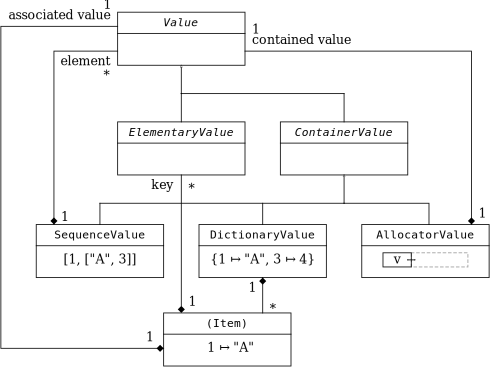
\includegraphics[scale=0.8]{classdiag_container}%
        \caption{Class hierarchy of container values.}
        \label{fig:class:ContainerValue}
    \end{quote}
\end{figure}


\subsubsection{\DborSequenceValue(\texorpdfstring{$v_1, \ldots, v_r$}{v1, ...m vr})}
%%%%%%%%%%%%%%%%%%%%%%%%%%%%%%%%%%%%%%%%%%%%%%%%%%%%%%%%%%%%%%%%%%%%%%%%%%%%%%%%%%%%
\hypertarget{sec:def:SequenceValue}{}

\paragraph{Representable objects}

A \DborSequenceValue{} can represent any sequence $v_1, \ldots, v_r$
of well-formed values (its elements) with the total size $\sum_{i = 1}^r \|v_i\| \in \IntegerInterval{0}{N + 23}$.

\paragraph{Representation}

A representable sequence $v_1, \ldots, v_r$ is represented as
\DborIntegerToken*($4$, $m$) {\Concat} $v_1 \Concat \cdots \Concat v_r$
with $m := \sum_{i = 1}^r \|v_i\|$.

\smallskip
\noindent
\begin{BeginParPenalty}
    Examples:
    \begin{quote}
        \noindent
        \begin{tabular}{lll}
            \toprule
            Value & Representation \\
            \midrule
            \DborSequenceValue()
                & \ByteSequence{\DborFirstByteHex{Sequence}{80}} \\
            \DborSequenceValue(\DborNoneValue, \DborIntegerValue($24$))
                & \ByteSequence{\DborFirstByteHex{Sequence}{83},
                        \DborFirstByteHex{None}{FF},
                        \DborFirstByteHex{Number}{18}, \DborNextByteHex{00}} \\
            \bottomrule
        \end{tabular}
    \end{quote}
\end{BeginParPenalty}

A non-empty byte sequence \ByteSequence{b_1, \ldots, b_n} is a \emph{size-correct} \DborSequenceValue{}
if and only if it is
\DborIntegerToken*($4$, $m$) {\Concat} \ByteSequence{b_{n - m + 1}, \ldots, b_n} for a suitable
$m \in \IntegerInterval{0}{N + 23}$.
It is a well-formed \DborSequenceValue{} if and only if it is a size-correct \DborSequenceValue{} and
\ByteSequence{b_{n - m + 1}, \ldots, b_n} is the concatenation of ($0$ or more)
well-formed values with a total size $m$.

The sequence is an \emph{ill-formed} \DborSequenceValue{} if and only if it is not a well-formed
\DborSequenceValue{} but $b_1$ is the first byte of an \DborIntegerToken*($4$, $m$).

\paragraph{Ambiguity, canonical value}

Whether there is more than one \DborSequenceValue{} representing the same object depends on its
elements.
The canonical value of \DborSequenceValue{}($v_1, \ldots, v_r$) is
\DborSequenceValue($v_1', \ldots, v_r'$)
where $v_i'$ is the canonical value of $v_i$ for all $i \in \IntegerInterval{1}{r}$.


\subsubsection{\DborDictionaryValue(\texorpdfstring{%
    $k_1 \mapsto v_1, \ldots, k_r \mapsto v_r$%
}{%
    k1 -> v1, ..., kr -> vr%
})}
%%%%%%%%%%%%%%%%%%%%%%%%%%%%%%%%%%%%%%%%%%%%%%%%%%%%%
\hypertarget{sec:def:DictionaryValue}{}

\paragraph{Representable objects}

A \DborDictionaryValue{} can represent any dictionary $k_1 \mapsto v_1, \ldots, k_r \mapsto v_r$ with
\begin{itemize}
    \item
    pairwise distinct, well-formed $k_i$ (its keys) that are instances of \DborElementaryValue
    \footnote{
        Comparision of keys is an important operation and must be fast.
        When the keys must be compared efficiently and the fill bytes in \DborAllocatorValue*{} must be
        ignored; a container value that can contain an \DborAllocatorValue*{} must be processed in depth
        which makes such a comparison operation complex and slow.
        Disallowing container values makes the comparison operation simple and fast.
    }
    and

    \item
    well-formed values $v_i$ (the values associated with $k_i$)

    \item
    with the total size $\sum_{i = 1}^r \big(\|k_i\| + \|v_i\|\big) \in \IntegerInterval{0}{N + 23}$ and

    \item
    $v_{i - 1} \prec v_{i}$ for all $i \in \IntegerInterval{2}{r}$.
\end{itemize}

${\prec}$ is the strict total order on the set of byte sequences defined in section~\ref{sec:stricttotalorder}.

\paragraph{Representation}

A representable dictionary $k_1 \mapsto v_1, \ldots, k_r \mapsto v_r$ is represented as
\DborIntegerToken*($5$, $m$) {\Concat} $k_1 \Concat v_1 \Concat \cdots \Concat k_r \Concat v_r$
with $m := \sum_{i = 1}^r \big(\|k_i\| + \|v_i\|\big)$.

\smallskip
\noindent
\begin{BeginParPenalty}
    Examples:
    \begin{quote}
        \noindent
        \begin{tabular}{lll}
            \toprule
            Value & Representation \\
            \midrule
            \DborDictionaryValue()
                & \ByteSequence{\DborFirstByteHex{Dictionary}{A0}} \\
            \DborDictionaryValue($\DborIntegerValue(24) \mapsto \DborNoneValue$)
                & \ByteSequence{\DborFirstByteHex{Dictionary}{A3},
                        \DborFirstByteHex{Number}{18}, \DborNextByteHex{00},
                        \DborFirstByteHex{None}{FF}} \\
            \bottomrule
        \end{tabular}
    \end{quote}
\end{BeginParPenalty}

A non-empty byte sequence \ByteSequence{b_1, \ldots, b_n} is a \emph{size-correct} \DborDictionaryValue{}
if and only if it is
\DborIntegerToken*($5$, $m$) {\Concat} \ByteSequence{b_{n - m + 1}, \ldots, b_n} for a suitable
$m \in \IntegerInterval{0}{N + 23}$.
It is a \emph{well-formed} \DborDictionaryValue{} if and only if it is a size-correct \DborDictionaryValue{} and
\begin{itemize}
    \item
    \ByteSequence{b_{n - m + 1}, \ldots, b_n} is the concatenation of an even number $2 r$ of
    well-formed values $k_1, v_1, \ldots, k_r, v_r$ with total size $m$, and

    \item
    the $k_1, \ldots, k_r$ are instances of \DborElementaryValue, and

    \item
    $v_{i - 1} \prec v_{i}$ for all $i \in \IntegerInterval{2}{r}$.
\end{itemize}

The sequence is an \emph{ill-formed} \DborDictionaryValue{} if and only if it is not a well-formed
\DborDictionaryValue{} but $b_1$ is the first byte of an \DborIntegerToken*($5$, $m$).


\paragraph{Ambiguity, canonical value}

Whether there is more than one \DborDictionaryValue{} representing the same object depends on its elements.
The canonical value of a well-formed \DborDictionaryValue($k_1 \mapsto v_1, \ldots, k_r \mapsto v_r$) is
the well-formed \DborDictionaryValue{} whose pairs of keys and associated values are the members of
$\{(k_i', v_i') \colon i \in I\}$ where $\Box'$ means the canonical value of $\Box$ and
$I := \{i \in \IntegerInterval{1}{r}\colon \min\{j \in \IntegerInterval{1}{r}\colon k_j' = k_i'\}\}$.

\medskip
Note:
The keys are formed by the bytes sequences, \emph{not} the represented objects.
It is therefore recommended to use only canonical values as keys.
\DborIntegerValue{}, \DborByteStringValue{}, and \DborUtfEightStringValue{} with code points $< \HexNumber{300}$
are especially well suited; they are all canonical and can easily be ordered according to
section~\ref{sec:stricttotalorder} \emph{before} encoding.


\subsubsection{\DborAllocatorValue(\texorpdfstring{$m$, $v$}{m, v})}
%%%%%%%%%%%%%%%%%%%%%%%%%%%%%%%%%%%%%%%%%%%%%%%%%%%%%%%%%%%%%%%%%%%%
\hypertarget{sec:def:AllocatorValue}{}

\paragraph{Representable objects}

An \DborAllocatorValue{} can represent the fixed-size allocation of a well-formed object~$v$
that is not an \DborAllocatorValue with $\|v\| \le m$ for $m \in \IntegerInterval{1}{N}$.

For all such $v$, $\|\DborAllocatorValue($m$,{} $v$)\|$ is independent of $\|v\|$.

\paragraph{Representation}

A representable \DborAllocatorValue($m$, $v$) is represented as
\DborNaturalToken*($6$, $0$, $m$) {\Concat} $v \Concat \ByteSequence{f_{\|v\| + 1}, \ldots, f_m}$
with arbitrary fill bytes $f_{\|v\| + 1}, \ldots, f_m$.

\smallskip
\noindent
\begin{BeginParPenalty}
    Examples:
    \begin{quote}
        \noindent
        \begin{tabular}{lll}
            \toprule
            Value & Representation \\
            \midrule
            \DborAllocatorValue(3, \DborIntegerValue(23))
                & \ByteSequence{\DborFirstByteHex{Allocator}{C0}, \DborNextByteHex{02},
                        \DborFirstByteHex{Number}{17},
                        \DborNextByteFillHex{FF}, \DborNextByteFillHex{FF}} \\
            \DborAllocatorValue(3, \DborIntegerValue(24))
                & \ByteSequence{\DborFirstByteHex{Allocator}{C0}, \DborNextByteHex{02},
                        \DborFirstByteHex{Number}{18}, \DborNextByteHex{00},
                        \DborNextByteFillHex{FF}} \\
            \bottomrule
        \end{tabular}
    \end{quote}
\end{BeginParPenalty}

A non-empty byte sequence \ByteSequence{b_1, \ldots, b_n} is a \emph{size-correct}
\DborAllocatorValue{} if and only if it is
\DborNaturalToken*($6$, $0$, $m$) {\Concat} \ByteSequence{b_{n - m + 1}, \ldots, b_n} for a suitable
$m \in \IntegerInterval{1}{N}$.
It is a \emph{well-formed} \DborAllocatorValue{} if and only if it is a size-correct \DborAllocatorValue{} and
\ByteSequence{b_{n - m + 1}, \ldots, b_n} is a well-formed value $v$ that is not an \DborAllocatorValue.

The sequence is an \emph{ill-formed} \DborAllocatorValue{} if and only if it is not a well-formed
\DborAllocatorValue{} but $b_1$ is the first byte of a \DborNaturalToken*($6$, $0$, $m$).

\paragraph{Ambiguity, canonical value}

Whether there is more than one \DborAllocatorValue{} representing the same object depends on its
contained element.
The canonical value of \DborAllocatorValue($m$, $v$) is
\DborAllocatorValue($m$, $v'$) where $v'$ is the canonical value of $v$
and all fill bytes $f_{\|v'\| + 1}, \ldots, f_m$ are $\HexNumber{FF}$.


\subsection{Strict total order}
%%%%%%%%%%%%%%%%%%%%%%%%%%%%%%%
\label{sec:stricttotalorder}

On the set of all byte sequences, ${\prec}$ induces a strict total order when defined as follows:

\paragraph{Definition}

For each pair of non-empty byte sequences
$a := \ByteSequence{a_1, \ldots, a_m}$,
$b := \ByteSequence{b_1, \ldots, b_n}$,
$a \prec b$ if and only if
\begin{itemize}
    \item $a_1 < b_1$, or
    \item $a_1 = b_1$ and $m < n$, or
    \item $a_1 = b_1$ and $m = n$ and $a_i < b_i$ where $i$ is the largest index
    $\in \IntegerInterval{2}{m}$ with $a_i \ne b_i$.
\end{itemize}
In addition: $\ByteSequence{} \prec a$ if and only if $a$ is a non-empty byte sequence.

\paragraph{Resulting order of values}
\begin{flushleft}
    $\ByteSequence{}
    \prec \DborIntegerValue(0) \prec \DborIntegerValue(1) \prec \dots \prec \DborIntegerValue(N + 23)
    \prec \DborIntegerValue(-1) \prec \DborIntegerValue(-2) \prec \dots \prec \DborIntegerValue(-(N + 24))
    \prec \DborByteStringValue(\ldots)
    \prec \DborUtfEightStringValue(\ldots)
    \prec \DborSequenceValue(\ldots)
    \prec \DborDictionaryValue(\ldots)
    \prec \DborAllocatorValue(\ldots)
    \prec \DborBinaryRationalValue(\ldots)
    \prec \DborDecimalRationalValue(\ldots)
    \prec \DborMinusZeroValue()
    \prec \DborMinusInfinityValue()
    \prec \DborInfinityValue()
    \prec \DborNoneValue()$.
\end{flushleft}
